\documentclass[tikz,border=5pt]{standalone}
\usetikzlibrary{arrows.meta,positioning}
\begin{document}
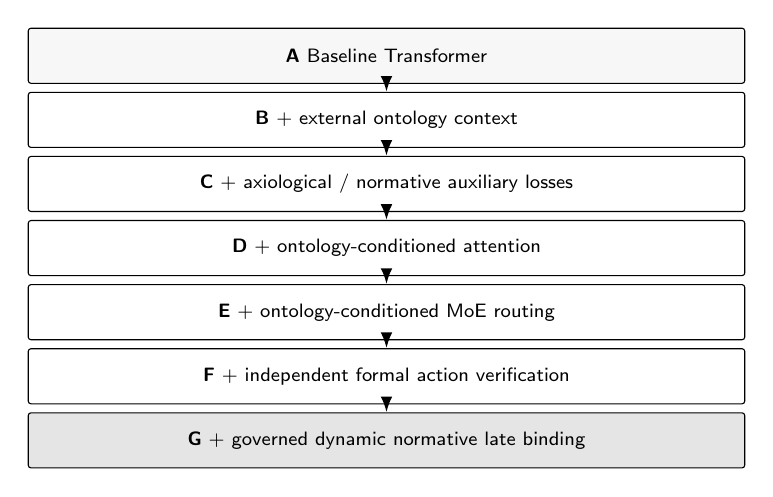
\begin{tikzpicture}[
  row/.style={draw, rounded corners=1pt, minimum width=91mm, minimum height=7mm, align=left, font=\sffamily\scriptsize, inner xsep=3mm},
  arrow/.style={-{Latex[length=2mm]}, thick}
]
\node[row, fill=black!3] (a) {\textbf{A} Baseline Transformer};
\node[row, below=1mm of a] (b) {\textbf{B} + external ontology context};
\node[row, below=1mm of b] (c) {\textbf{C} + axiological / normative auxiliary losses};
\node[row, below=1mm of c] (d) {\textbf{D} + ontology-conditioned attention};
\node[row, below=1mm of d] (e) {\textbf{E} + ontology-conditioned MoE routing};
\node[row, below=1mm of e] (f) {\textbf{F} + independent formal action verification};
\node[row, below=1mm of f, fill=black!10] (g) {\textbf{G} + governed dynamic normative late binding};
\draw[arrow] (a) -- (b);
\draw[arrow] (b) -- (c);
\draw[arrow] (c) -- (d);
\draw[arrow] (d) -- (e);
\draw[arrow] (e) -- (f);
\draw[arrow] (f) -- (g);
\end{tikzpicture}
\end{document}
